% Created 2016-02-24 Wed 09:09
\documentclass[9pt,b5paper]{article}
\usepackage{graphicx}
\usepackage{xcolor}
\usepackage{xeCJK}
\setCJKmainfont{SimSun}
\usepackage{longtable}
\usepackage{float}
\usepackage{textcomp}
\usepackage{geometry}
\geometry{left=0cm,right=0cm,top=0cm,bottom=0cm}
\usepackage{multirow}
\usepackage{multicol}
\usepackage{listings}
\usepackage{algorithm}
\usepackage{algorithmic}
\usepackage{latexsym}
\usepackage{natbib}
\usepackage{fancyhdr}
\usepackage[xetex,colorlinks=true,CJKbookmarks=true,linkcolor=blue,urlcolor=blue,menucolor=blue]{hyperref}


\lstset{language=c++,numbers=left,numberstyle=\tiny,basicstyle=\ttfamily\small,tabsize=4,frame=none,escapeinside=``,extendedchars=false,keywordstyle=\color{blue!70},commentstyle=\color{red!55!green!55!blue!55!},rulesepcolor=\color{red!20!green!20!blue!20!}}
\author{deepwaterooo}
\date{\today}
\title{AI Connect Four}
\hypersetup{
  pdfkeywords={},
  pdfsubject={},
  pdfcreator={Emacs 24.3.1 (Org mode 8.2.7c)}}
\begin{document}

\maketitle
\tableofcontents


\section{On processing Mini-max algorithm with Alpha-beta pruning for Connect 4 game human vs AI.}
\label{sec-1}
\begin{itemize}
\item Status now: GUI almost there, need to rewrite AI using Java. 

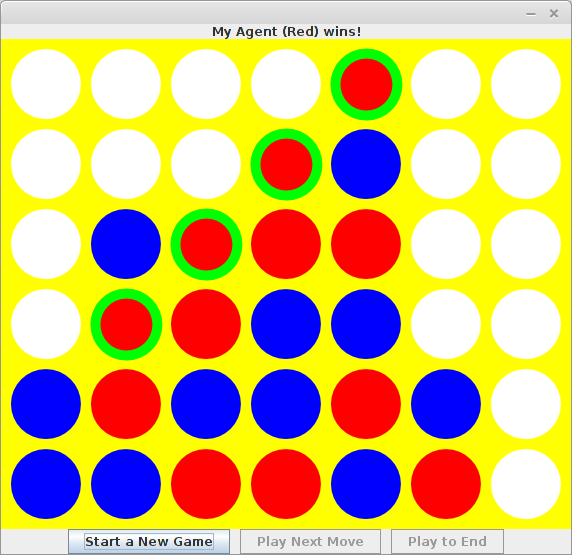
\includegraphics[width=.9\linewidth]{./connect4.png}
\end{itemize}

\section{Rules of the Game}
\label{sec-2}

\begin{itemize}
\item To what type of object will you add an instance of a PlayListener object (as a Mouse-Listener)?

\item If your board has w columns and h rows, how many BoardCell objects do you need to create?   To which component will you add these BoardCell objects?

\item Why is the JLabel status an instance variable (as opposed to just a local variable in the constructor)?

\item Where is the information about what contents are stored in each cell located?  What method must the BoardCell call in its paintComponent method to determine what color to paint the "checker"?

\item Which method will determine when the game is over (by calling methods on the ConnectFourBoard object theBoard)?  Which method will detect illegal moves (again by calling methods on the ConnectFourBoard object theBoard)?

\item Will you need to create a separate listener to handle clicks on the New Game button, or will you use another instance of the PlayListener class?

\item How do you run the game?
\end{itemize}

\section{The Project Architecture}
\label{sec-3}
\begin{itemize}
\item Will fill diagrams later
\end{itemize}

\section{Designing Your Agent}
\label{sec-4}
\begin{itemize}
\item One AI
\item One human player
\end{itemize}

\section{Playing Your Agent}
\label{sec-5}
\begin{itemize}
\item Either human or AI can play first
\begin{itemize}
\item Let AI to play a move by clicking "Next Move" button
\item Human play by clicking the mouse into a specific column
\end{itemize}
\end{itemize}

\section{Further Reading}
\label{sec-6}

\section{Prefix}
\label{sec-7}
\begin{itemize}
\item The original Connect 4 AI project was written and finished by Mar 5, 2013, which was my second semester for Computer Science major, so there are lots of defects.
\item This is a game rewrite using Java to build a graphic interface following major requirements from the initial course project requirements, and UCSD PSA6: Connect 4 GUI requirements, whose reference is listed below.
\item This is the very FIRST Java project that I built (design was still pretty much there by surfing internet) except the Android App Projecting DrawingFun app, which project's frame work was almost pretty much there and I just added functionality.
\end{itemize}

\section{references}
\label{sec-8}
\begin{itemize}
\item mouselistener:
\begin{itemize}
\item \url{https://www.youtube.com/watch?v=TMWUZ5vzghc}
\item \url{http://bbs.csdn.net/topics/320055502}, this one works!
\end{itemize}
\item requirements
\begin{itemize}
\item \url{https://sites.google.com/a/eng.ucsd.edu/cse-8b-winter-2014/schedule-and-assignments/psa6}
\item \url{https://github.com/lisalisadong/cs-046}
\end{itemize}
\end{itemize}
% Emacs 24.3.1 (Org mode 8.2.7c)
\end{document}